\section{Beschneidung des Netzes zur Beschleunigung des Training}
\label{sec:prunetrain}
Das Beschneiden\footnote{Beschneiden wird hier äquivalent zum Englischen  "`to prune"' verwendet} des Netzes ist eine Technik, die entwickelt wurde, um die Inferenzzeit eines neuronalen Netzwerks zu reduzieren. Das Beschneidungsverfahren wird auf das bereits trainierte Netz angewendet. Dabei wird entschieden, welche Gewichte nur einen minimalen oder keinen Effekt auf das Klassifikationsergebnis haben, um diese zu entfernen.

Das Beschneiden des Netzes kann auch verwendet werden, um die Trainingszeit zu minimieren. Diese Methode soll in diesem Unterkapitel erläutert werden. Als Quelle für dieses Unterkapitel dient ein Paper, welches evaluiert inwiefern Trainingszeit mittels Beschneiden gespart werden kann \cite{prunetrain}.


Das Ziel des Beschneidens während dem Training ist es, die Gewichte einzelner Kanäle auf Null zu setzen und zu entfernen, um mit einem kleinerem Netz in den nachfolgenden Epochen Trainingszeit zu sparen. Dazu wird der Verlust-Funktion des Netzwerks ein Normalisierungsterm addiert. Damit die Gewichte ganzer Kanäle möglichst unter den Schwellwert fallen werden die Gewichte der Kanäle gemeinsam quadriert, wie in der folgenden Gleichung zu sehen ist:

\begin{equation}
GL(\mathcal{W})=\sum_{g=1}^{G} \left( \sum_{c_g=1}^{C_g} || W_{g} (c_g,:,:,:) ||_2 + \sum_{k_g=1}^{K_g} || W_{g}(:,k_g,:,:)||_2 \right)
 \label{equ:PTloss}
\end{equation}

Dieser Term nennt sich Gruppen-Lasso. Der Parameter $W_{g}$ stellt die Gewichte im CNN als Tensor dar. Mit $g$ wird dargestellt um welches Layer es sich handelt. Die Dimensionen des Tensors sind: Ausgangskanäle \texttimes Eingangskanäle \texttimes Kerneldimension 1 \texttimes Kerneldimension 2. $G$ gibt an über wie viele Layer der Gruppen-Lasso Term berechnet wird. $k_g$ ist die Laufvariable über die einzelnen Eingangskänale und $c_g$ über die einzelnen Ausgangskanäle. Alternativ zum Gruppen-Lasso Regularisierer könnten hier auch andere Regularisierer, wie L1 bzw. L2 Regularisierer verwendet werden. Der Vorteil des Gruppen-Lasso Regularisierers ist, das durch das gemeinsame Quadrieren der Gewichte einer Schicht diese gemeinsam minimiert werden.


Um das Verhältnis von Gruppen-Lasso Term zur Verlust-Funktion dynamischer wählen zu können, werden diese nicht einfach aufeinander addiert. Es wird abhängig von der Initialbelegung der Gewichte ein Parameter $\lambda$  berechnet, der Gruppen-Lasso und Verlust-Funktion balanciert:

\begin{equation}
 LPR\left(GL(\mathcal{W}),l(f(\mathbf{x}_i,\mathcal{W}),y_i)\right) = \frac{\lambda \cdot GL(\mathcal{W})}{l(f(\mathbf{x}_i,\mathcal{W}), y_i) + \lambda \cdot GL(\mathcal{W})}           
\end{equation}

Die Größe LPR ist hier echt zwischen Null und Eins wählbar. Je größer sie gewählt wird, desto größer ist der Anteil, der beschnitten wird. Regelmäßig werden während dem Trainieren des Netzes Gewichte, die unter dem Schwellwert liegen auf Null gesetzt. Es entsteht ein nur dünn besetztes Netz. Dann wird durch ein Rekonfigurationsverfahren aus dem dünn besetzten Netz ein dicht besetztes Netz ohne die vorher nicht besetzten Kanäle. Um dieses Verfahren durchzuführen muss überprüft werden, ob mit dem Entfernen der Kanäle die Dimensionen der verschiedenen aufeinanderfolgenden Kanäle übereinstimmen. Bei einem residualen Netz muss zusätzlich darauf geachtet werden, dass die Dimensionen der Kurzschluss-Verbindungen zusammen passen.

\todo[inline,color = blue]{Grafik zum Verfahren}

Zu diesem Zweck wird das Kanal-Union Verfahren eingeführt. Beim Kanal-Union Verfahren wird ein Liste mit den Layern geführt, die aufeinander abgestimmt werden müssen. Im Falle eines residualen Netzes muss zusätzlich eine Liste über die zusammengehörigen Layer der Kurzschlussverbindungen geführt werden. Im nächsten Schritt werden alle Eingangs- und Ausgangskanäle, die noch Gewichte größer Null haben in einer Liste gesammelt. Auf allen Elementen dieser Liste wird nun geprüft, ob mit Hilfe von Vereinigungen Kanäle gefunden werden können die zwar keine von Null verschiedenen Gewichte mehr haben, wegen der Dimensionalität aber trotzdem beibehalten werden müssen. Alle Kanäle die nicht unter diese Bedingung fallen können mit Hilfe einer Rekonfiguration aus dem Netzwerk entfernt werden. 

\todo[inline, color = blue]{Noch genauer formulieren}
\begin{figure}[htbp]
\fcolorbox{red}{white}{
\begin{minipage}[t]{0.35\textwidth}
\vspace{0pt}
\centering
 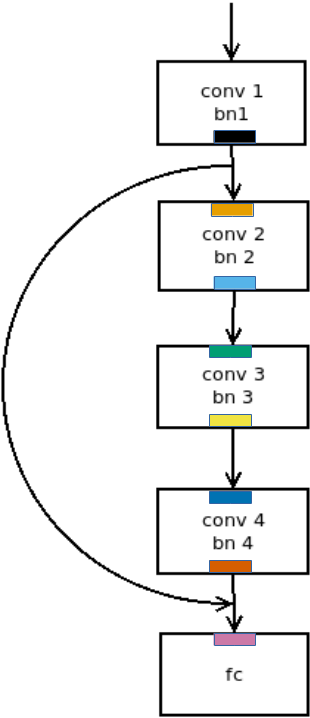
\includegraphics[width=0.9
 \textwidth]{KapitelPartA/images/net.png}
 % net.pdf: 0x0 px, 300dpi, 0.00x0.00 cm, bb=
 \caption{Beispielnetz}
 \label{abb:cu}
\label{fig:Bild1}
\end{minipage}
\hfill
\begin{minipage}[t]{0.65\textwidth}
\vspace{0pt}

Liste der Layer, die direkt hintereinander sind und aufeinander abgestimmt werden müssen (ohne das zwischen den Layern eine Kurzschlussverbindung enstammt oder endet): $H=\left\{(2,3),(3,4) \right\}$


Liste der Layer, die im Zusammenhang mit den Kurzschlussverbindungen die gleiche Eingangskanaldimension haben müssen: $E=\left\{(2,fc \right\}$

Liste der Layer, die im Zusammenhang mit den Kurzschlussverbindungen die gleiche Ausgangskanaldimension haben müssen: $A=\left\{(1,4 )\right\}$

Liste der dicht-besetzten Schichten vor dem ersten Beschneiden:\\
$1:\left\{0,1,2\right\},\left\{0,1,2,3,4,5,6,7\right\}$\\ 
$2:\left\{0,1,2,3,4,5,6,7\right\},\left\{0,1,2,3,4,5,6,7\right\}$\\
$3:\left\{0,1,2,3,4,5,6,7\right\},\left\{0,1,2,3,4,5,6,7\right\}$\\
$4:\left\{0,1,2,3,4,5,6,7\right\},\left\{0,1,2,3,4,5,6,7\right\}$\\
$fc:\left\{0,1,2,3,4,5,6\right\},\left\{0,1,2,3,4,5,6,7,8,9,10\right\}$\\

Liste der dicht-besetzten (db) Schichten nach dem auf Null setzen der Parameter aber vor der Rekonfiguration:\\
$1:\left\{0,1,2\right\},\left\{0,1,4,5,6,7\right\}$\\ 
$2:\left\{0,1,3,5,6,7\right\},\left\{0,1,2,4,5,6,7\right\}$\\
$3:\left\{0,1,2,4,5,6,7\right\},\left\{0,1,2,3,4,5,6,7\right\}$\\
$4:\left\{0,1,2,3,4,6,7\right\},\left\{0,1,3,4,5,6,7\right\}$\\
$fc:\left\{0,1,3,4,5,6\right\},\left\{0,1,2,3,4,5,6,7,8,9,10\right\}$\\

Vorgehen des Kanal Union Verfahren:
Als ersten Schritt wird für alle Elemente aus $H$ die Vereinigung von Ausgangs-und Eingangskanälen berechnet und diese dann zugewiesen:\\
$2,3:A(2) \cup E(3)= \l\left\{0,1,2,4,5,6,7\right\} \cup \left\{0,1,2,4,5,6,7\right\} =\left\{0,1,2,4,5,6,7\right\} $\\ Hier wird der dünn-besetzte Kanal 3 entfernt\\
$3,4: A(3) \cup E(4) =
\left\{0,1,2,3,4,5,6,7\right\} \cup :\left\{0,1,2,3,4,6,7\right\} = \left\{0,1,2,3,4,5,6,7\right\}$\\
Der nullwertige Eingangskanal 5 von Schicht 4 wird nicht entfernt, da der dazugehörige Ausgangskanal von Schicht 3 nicht nullwertig ist.

Im nächsten Schritt werden für die Elemente an jeweils gleicher Stelle aus den Mengen A und E Vereinigungen gebildet:\\
$A(1)\cup A(4) \cup E(2) \cup E(fc)=\\
\left\{0,1,4,5,6,7\right\} \cup \left\{0,1,3,4,5,6,7\right\} \cup \left\{0,1,3,5,6,7\right\} \cup \left\{0,1,3,4,5,6\right\} = \left\{ 0,1,3,4,5,6,7\right\}$
Hier wir in den Ausgangskanälen von Schicht 1 und 2 sowie in den Eingangskanälen von Schicht 2 und fc jeweils der 2. Kanal entfernt.

\end{minipage}
}
\caption{Beispiel für das Kanal-Union Verfahren}

\end{figure}



Bei einem residualen Netzwerk ist es weiterhin möglich, dass ein ganzer Block wegfällt. In diesem Fall müssen die Kanal-Union Listen angepasst werden und es wird mit einem ohne diesen Block um mehrere Layer verkürztes Netzwerk weitergemacht.


Da mit dem Verkleinern des Netzes nicht nur potentiell Zeit sondern auch Speicherplatz gespart wird, kann bei gleicher Speicherauslastung die Batchgröße erhöht werden. Da die verwendete Technik für die Erhöhung der Batchgröße in der Quelle nicht angegeben ist und in der verwendeten Implementierung fehlt wurde diese nachimplementiert und wird in Kapitel \ref{sec:ptEva} erläutert \cite{ptImpl}. Hierbei wird die Lernrate an die erhöhte Batchgröße angepasst um negative Effekte für die Accuracy abzumildern oder auszuschließen. 

Damit lassen sich Netzverkleinerungsraten von etwa 50 \% erreichen bei weniger als 2 \% Accuracy-Verlust auf dem Datensatz Cifar10. Andere Techniken schaffen zwar zwischen 70 - 80 \% Netzverkleinerungsraten brauchen aber wesentlich mehr Trainingszeit \cite{lottery}. Diese großen Verkleinerungsraten sind dort sehr stark abhängig von der Initialisierung \cite{lottery}. Das heißt nur einzelne Initialisierungen führen zu so starken Verkleinerungsraten, was insgesamt zu einer längeren Trainingszeit führt \cite{lottery}. 


Eine weitere Beschneidungstechnik arbeitet vor dem Training des Netzwerkes\cite{snyc}. Damit wird das Netz abhängig von der Initialbelegung beschnitten. Es lassen sich zwar sehr große Teile der Parameter auf Null setzen, hierbei wird im Vergleich zur Beschneidungsmethode währenddem Training allerdings weder für gemeinsames Beschneiden von Kanälen gesorgt, noch wird ein Rekonfigurationsverfahren vorgestellt. Somit hat das Netz am Ende des Verfahrens zwar relativ viele auf Null gesetzte Parameter ist aber weder schneller noch kleiner.


\section{Beschleunigung des Lernens durch Wissenstransfer}
\label{sec:net2net}
Beim Trainieren eines CNNs kommt es häufig vor, dass nach initialem Wählen der Tiefe bzw. Breite des Netzes diese Parameter in einem weiteren Trainingslauf erhöht werden und in Folge dessen das Netzwerk komplett neu trainiert werden muss. Mit Hilfe der Quelle zu diesem Unterkapitel wurde ein Verfahren geschaffen, welches das Netz tiefer oder breiter machen kann und dabei die im ersten Trainingsdurchlauf trainierten Gewichte weiter verwendet \cite{net2net}. Durch diesen Wissenstransfer von einem Netz zu einem tieferen oder breiteren Netz wird eine schnellere Konvergenz des neuen Netzes erwartet. Durch die Initialisierung mit schon vorhandenen Parametern entsteht eine Transformation, die die erlernte Funktion erhält.

\begin{figure}[h]
 \centering
 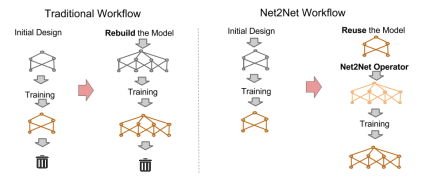
\includegraphics[width=0.7\textwidth]{KapitelPartA/images/net2net.png}
 % net2net.png: 433x179 px, 72dpi, 15.28x6.31 cm, bb=0 0 433 179
 \caption{Traditioneller Workflow vs. Net2Net Workflow}
 \label{abb:net2net}
\end{figure}


Wie in Abbildung \ref{abb:net2net} abgebildet ist lässt sich so der Workflow zum Finden der passenden Netzstruktur anders gestalten. Der Net2Net Operator macht dabei das Netz entweder breiter (mehr Kanäle in bestimmten Schichten) oder tiefer (zusätzliche Schichten). Diese beiden Operatoren werden nun vorgestellt.

\subsection{Operator für breiteres Netz}
Bei dem Net2Net-Operator, der das Netz breiter macht werden für eine bestimmte Schicht Ausgangskanäle und für die nachfolgende Schicht Eingangskanäle hinzugefügt. Die Schicht, der Ausgangskanäle hinzugefügt werden wird mit $g$ bezeichnet und hat den Gewichtstensor $\mathbf{W}_g$ mit der Dimensionalität von $n \times l \times d(h_{l,1}) \times d(h_{(l,2)}$. Die Schicht, der Eingangskanäle hinzugefügt werden wird mit $g+1$ bezeichnet und hat den Gewichtstensor $\mathbf{W}_{g+1}$ mit der Dimensionalität von $m \times n \times d(f_{g+1,1}) \times d(h_{g+1,2})$. Dem Layer $g$ werden $q$ Kanäle hinzuefügt. Dies entspricht wie in Abbildung \ref{abb:channels} abgebildet ist $q \cdot l $ zusätzlichen Filterkerneln. 
\begin{figure}[h]
 \centering
 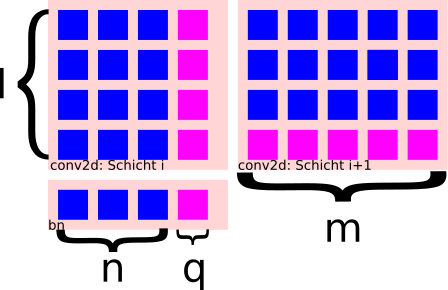
\includegraphics[width=0.6\textwidth]{KapitelPartA/images/channels.png}
 % channels.pdf: 0x0 px, 300dpi, 0.00x0.00 cm, bb=
 \caption{Übersicht über die zusätzlichen Kanäle todo: Grafik schön machen}
\label{abb:channels}
 \end{figure}



Für das Layer $g+1$ sind es entsprechend $q \cdot m $ zusätzliche Kernel. Die Gewichtstensoren nachdem Anwenden des Net2Net Operators werden mit $\mathbf{U}^i$ und $\mathbf{U}^{i+1}$ bezeichnet und sollen die Dimensionalität von $\mathbf{U}^i: (n+q) \times l \times d(f_{(i,1)}) \times d(f_{(i,2)})$ und $\mathbf{U}^{i+1}: m \times (n+q) \times d(f_{(i+1,1)}) \times d(f_{(i+1,2)})$ haben. Der Net2Net Operator wird angewendet, indem zunächst eine Mapping Funktion $g$ definiert wird die für ein zufällige Belegung der zusätzlichen Kernels sorgt:

\begin{equation}
 g_{j} =  
 \begin{cases}
 j & , \text{ falls} \, j \leq n \\
 k & , \text{ falls} \, j>n : \;  k \text{ zufälliges Sample von} \left\{ 1,2,\ldots, n \right\} \\ 
 \end{cases} 
 \end{equation}
 Mit Hilfe dieser Mapping-Funktion werden nun die neuen Gewichtstensoren initialisiert:
 \begin{equation}
 \mathbf{U}^i_{j,k,f_1,f_2} = \mathbf{W}^i_{g(j),k,f_1,f_2} \; \; \mathbf{U}^{i+1}_{h,j,f_3,f_4}= \frac{1}{|\left\{ x | g(x)=g(j)\right\}|}\mathbf{W}^{i+1}_{h,g(j),f_3,f_4}
 \end{equation}
Die Funktion $g(j)$ wird dabei für jede neu hinzugekommene Schicht nur einmal ausgewertet, sodass gesamte Reihen statt einzelne Kernel kopiert werden. Sollte sich zwischen dem $i$-ten und $(i+1)$-Layer eine Batchnormalisierung befinden, so werden die Parameter dieser Schicht ebenfalls kopiert.

Um nicht mehrere exakt gleiche Kernelreihen zu haben kann außerdem noch ein Noiseanteil auf alle neuen Gewichte addiert werden. Dies ist vor allem für den Fall wichtig, wenn der Trainingsalgorithmus keine Form der Randomiesierung hat, die gleichen Gewichtstensoren ermutigt unterschiedliche Funktionen zu erlernen. Somit sind die vom ursprünglichen und neuen Netz gelernten Funktionen ähnlich aber nicht gleich.

\subsubsection{Tieferes Netz}

Der Net2Net- Operator für ein tieferes Netz ersetzt die Operation der $i$-ten Schicht $\mathbf{h}^{(i)} = \phi\left(\mathbf{h}^{(i-1)t} \mathbf{W}^{(i)}\right)$ durch die Operation von zwei Layern  
\begin{equation}
\mathbf{h}^{(i)} = \phi( \mathbf{U}^{(i)t} \phi(\mathbf{W}^{(i)t}  \mathbf{h}^{(i-1}) )
\end{equation}
$\mathbf{U}$ wird als Identitätsmatrix initialisiert. Um die geforderte Erhaltung der gelernten Funktion zu erhalten muss für die Aktivierungsfunktion $\phi$ und alle Vektoren $\mathbf{v}$ die Gleichung $\phi(\mathbf{I} \phi(\mathbf{v}))=\phi(\mathbf{v}))$. Die Aktivierungsfunktion ReLu erfüllt diese Anforderung.

Wird zwischen den beiden Layern eine Batchnormalisierung genutzt, so müssen die Parameter der Batchnormalisierung so gewählt werden, dass sie die gelernte Funktion des Netzes nicht verändert.


\subsubsection{Diskussion der Methode}

Die beiden Net2Net-Operatoren schaffen die Möglichkeit Familien von Netzarchitekturen zu erforschen ohne jedes Mal von neuem zu lernen. Mit Hilfe der beiden Operatoren lässt sich die Komplexität des Netzes erhöhen ohne die gelernte bisherige Funktion zu vernachlässigen.


\section{Schnelles Ressourcen beschränktes Strukturlernen tiefer Netzwerke}\label{sec:morphnet}
Im Gegensatz zu den Kapiteln \ref{sec:prunetrain} und \ref{sec:net2net} , in denen jeweils eine Möglichkeit ein CNN kleiner sowie größer zu machen vorgestellt wurden geht es jetzt darum dies zu kombinieren. Die Quelle für diese Kapitel ist soweit nicht anders gekennzeichnet das Paper, welches die Methode vorgestellt hat \cite{morphnet}.

Die manuelle Wahl von Hyperparametern, die bestimmen wie groß und komplex ein neuronales Netz ist, braucht eine gewisse Kunstfertigkeit. Sind die Hyperparameter falsch gewählt, so müssen diese angepasst und das Netz erneut trainiert werden. Mit Hilfe der hier vorgestellten Methode wird diese Suche nach der besten Architektur automatisiert. Dies geschieht mit Hilfe von iterativen Verkleinern und Vergrössern des Netzes. Diese Methode hat drei Vorteile:
\begin{enumerate}
 \item Es ist auf große Netze und große Datensätze skalierbar
 \item Es kann die Struktur in Bezug auf eine bestimmte Nebenbedingung (zum Beispiel Modellgröße, Anzahl an Parametern) optimieren
 \item Es kann eine Struktur lernen, die die Performance erhöht
\end{enumerate}

Das Ziel der Methode ist es, automatisch die beste Architektur für ein Netz zu finden. Dies umfasst die Breiten der Eingangs- und Ausgangskanäle, Größe der Kernel, die Anzahl der Schichten und die Konnektivität dieser Schichten. Im Rahmen dieser Methode wird dies auf die Breite der Ausgangskanäle eingeschränkt. Die Methode kann auf die anderen Größen erweitert werden. Allerdings ist die Einschränkung auf die Breite der Ausgangskanäle sowohl effektiv als auch simpel.
Die Breite der Ausgangskanäle für alle $L$ Schichten wird mit $c_l$ bezeichnet. 

Der Anfangspunkt dieser Methode ist ein Netz $\mathcal{W}^1$ mit einer initialen Breite der Ausgangskanäle sowie fixen Größen für die Filtergrößen. Die Nebenbedingung wird mit der Funktion $\mathcal{F}$ bezeichnet. Sie optimiert entweder die Modellgröße oder die Anzahl an Flops per Inferenz. Die Methode optimiert formal gesehen also folgendes:
\begin{equation}
 \mathcal{W}^{\ast}_{1:L}= \underset{\mathcal{F}(c_l)\leq \zeta}{\text{arg min}} \underset{\theta}{\text{ min}}\; l(f(\mathbf{x_i}),y_i)\label{equ:morph1}
\end{equation}

Das Vergrößern des Netzes basiert auf einer Lösung für die Gleichung \ref{equ:morph1}: dem Breitenmultiplikator $\omega$. 
Sei $\omega \cdot O_{1:M} = \left\{ \lfloor \omega O_1 \rfloor, \lfloor \omega O_2 \rfloor, \ldots , \lfloor \omega O_M \rfloor \right\}, \omega>0$. Gilt $\omega>1$, so wird das Netz vergrößert. Bei $\omega <1$ wird das Netz verkleinert. Um die Gleichung \ref{equ:morph1} zu lösen finde nun das größte $\omega$, so dass $\mathcal{F}(\omega \cdot O_{1:M})\leq \zeta$ gilt.


Dieser Ansatz sorgt zwar für eine mögliche Verkleinerung und Vergrößerung des Netzes und er funktioniert gut bei einem guten initialen Netz. Ist das initialen Netz nicht von so guter Qualität, so hat dieser Ansatz Probleme. 
Dieser Nachteil wird durch eine Veränderung der Verlust-Funktion aufgehoben. Es wird ein Regularisierer dazu addiert, welcher die Kontribution eines Netzbestandteiles zu $\mathcal{F}( O_{1:M})$ misst und es damit direkt optimieren kann. Dann ist
\begin{equation}
 O^{\ast}_{1:M}= \underset{\mathcal{F}(O_{1:M})\leq \zeta}{\text{arg min}} \underset{\theta}{\text{min}}\; \mathcal{L}(\theta) + \lambda \mathcal{G}(\theta)  
 \label{equ:morph2}
\end{equation}
Dieser Ansatz kann die relative Größe eines Layers ändern, hat aber den Nachteil das häufiger die zu optimierende Nebenbedingung nicht maximal maximiert wird.




Die beiden Ansätze lassen sich kombinieren. Es entsteht folgender Algorithmus:
\begin{algorithm}[H]
\caption{MorphNet Algorithmus}
\begin{algorithmic}[1]
\STATE Trainiere das Netz um $f(\mathbf{x_i})^{\ast}=\underset{\theta}{arg min} \mathcal{L}(\theta) + \lambda \mathcal{G}(\theta)$ zu finden
\STATE Finde die neue Breite $O_{1:M}^{\prime}$, die durch 1. errechnet wurde
\STATE Finde das größte $\omega$, so dass $\mathcal{F}(\omega \cdot O_{1:M})\leq \zeta$ gilt
\STATE Wiederhole ab 1. so häufig wie gewünscht mit $O_{1:M} = O_{1:M}^{\prime}$
\ENSURE $\omega \cdot O_{1:M}$
\end{algorithmic}
\label{alg:morphnet}
\end{algorithm}
Dieser Algorithmus kann so oft durchlaufen werden bis entweder die Performance des Netzes gut genug ist, oder bis die letzten Durchläufe keine Veränderungen mehr hervorgebracht haben.


\subsection{Definition der Nebenbedingung}
Die Nebenbedingung $\mathcal{F}$ lässt sich für verschiedene zu optimierende Zielgrößen definieren. Eine einfache Nebenbedingungen, die Modellgröße wird hier beispielhaft erläutert. Die Größe dieser Nebenbedingung wird vorallem durch Schichten mit Matrixmultiplikation dominiert. Die Modellgröße ergibt sich durch die Größe der Tensoren der einzelnen Schichten. Da die Größe der Tensoren der einzelnen Schichten abhängig von der Anzahl der Eingangs- und Ausgangskänäle sowie der Filtergrösse sind und nicht von der Position im Netzwerk ist, lässt sich $\mathcal{F}(O_{1:M})$ auf die einzelnen Schichten zurückführen. Es gilt:
\begin{equation}
 \mathcal{F}(O_{1:M})=\sum_{L=1}^{M+1} \mathcal{F}(\text{layer} L)
\end{equation}
Für den Breitenmultiplikator $\omega$ gilt: $\mathcal{F}(\omega \cdot O_{1:M})=\omega \cdot \mathcal{F}(O_{1:M})$

Die Abhängigkeit von der Größe des jeweiligen Tensors ergibt für 
\begin{equation}
\mathcal{F}(\text{layer} L)=I_L \cdot O_L \cdot d(f_{L,1}) \cdot d(f_{L,2})  
\end{equation}
Da auf durch die Anwendung des Regularisierers einzelne Kanäle auf Null gesetzt werden und ein Netz ohne diesen Kanal möglich wären sollen diese Kanäle in dieser Berechnung ausgelassen werden. Daher wird die Formel um Aktivierungsfunktionen ergänzt die mit einer Eins angeben, dass der zugehörige Kanal nicht null ist. Eine Null als Ergebnis der Aktivierungsfunktion ergibt sich, wenn der entsprechende Kanal komplett auf Null gesetzt wurde. Es ergibt sich:
\begin{equation}
\mathcal{F}(\text{layer} L)=\left(\sum_{i=1}^{I_L} A_{L,i} \right) \cdot \left(\sum_{j=1}^{O_L} B_{L,j}\right) \cdot d(f_{L,1}) \cdot d(f_{L,2})  
\end{equation}


\subsection{Regularsierer}
Beim Verkleinern des Netzes soll die Verlustfunktion $\mathcal{L}$ des CNN mit der Nebenbedingung $\mathcal{F}(O_{1:M})\leq \zeta$ minimiert werden. Bei der Wahl des Regularisierers muss bedacht werden, dass der Regularisierer und seine Ableitung kontinuierlich definiert sein müssen, da die Parameter im Netz durch ein Gradientenabstiegsverfahren gelernt werden. Zusätzlich kann eine Nebenbedingung nicht direkt durch ein Gradientenabstiegsverfahren gelernt werden. Daher wird $\mathcal{F}$ in veränderter Form als Regulariser gewählt. Die Veränderung umfasst das Hinzufügen von $\gamma_L$, die ähnlich einer Batchnormalisierung genutzt werden:
\begin{equation}
\mathcal{G}(\theta, \text{layer} L)=\left(\sum_{i=1}^{I_L-1} A_{L,i} \sum_{j=0}^{O_{L}-1} |\gamma_{L,j} | \right) \cdot \left(\sum_{i=0}^{I_{L}-1} |\gamma_{L-1,i} |   \sum_{j=1}^{O_L-1} B_{L,j}\right) \cdot d(f_{L,1}) \cdot d(f_{L,2})  
\end{equation}

Mit dieser Funktion lässt mittels Gradientenabstieg lernen, obwohl Teile des Regularisieres nicht komplett kontinuierlich sind. Werden die $\gamma$ für einen Kanal auf Null gesetzt durch das Lernen, so ist der dazugehörige Kanal aus der Berechnung wie gewünscht ausgeschlossen. Aus dem Regularisierer einer Schicht lässt sich mittels Addition die Regularisierung des konpletten Netzes berechnen.
\begin{equation}
 \mathcal{G}(\theta)=\sum_{L=1}^{M+1} \mathcal{G}(\theta,layer L)
\end{equation}


Um die Wichtigekeit vom besseren Training des Netzes und der Regularisierung von Parametern treffen zu können wird ein Parameter $\lambda$ eingeführt. So entsteht die Verlust-Funktion
\begin{equation}
 \theta^{\ast}=\underset{\theta}{arg min} \mathcal{L}(\theta) + \lambda \mathcal{G}(\theta)
\end{equation}



Dieser Regularisierer funktioniert nicht für Netze, die Kurzschlussverbindungen besitzen. Hier wird wie bei Beschneiden des Netzes während dem Training die ein Gruppen-Lasso verwendet. Dies stellt sicher, dass an Kurzschlussverbindungen nur so beschnitten werden kann wie für die Dimensionalität des Netzes zuträglich.



\section{Automatische Architektursuche}\label{sec:auto}
Neben dem im letzen Kapitel ausführlich erläuterten Ansatz des Strukturlernens gibt es noch einige andere aktuelle Ansätze, die automatisch nach einer besseren Architektur für einen Datensatz suchen. Einige dieser Ansätze werden hier beleuchtet und es wird gezeigt, wieso das im letzten Kapitel erläuterte Verfahren im praktischen Teil weiter verwendet wird.

Bei dem Versuch die Hyperparameter eines Netzes sinnvoll automatisch zu wählen entsteht ein sehr großer Suchraum. Dieser Suchraum lässt sich mit viel Aufwand absuchen \cite{dvolver}. Es entsteht ein Optimierungsproblem mit mehreren zu optimierenden Variablen bei welchem eine Pareto-Front gesucht wird \cite{dvolver}. Das Ergbnis schafft eine Verbesserung der Accuracy gegenüber bekannten Architekturen, dabei summiert sich allerdings die Trainingszeit mit 20 NVIDIA V100 Grafikkarten für Imagenet auf 2,5 Tage\cite{dvolver}.

Ohne Einschränkung des Suchraumes sondern durch Einschränkung der Domain:
 



